\chapter{Resultados}\label{cap:Resultados}

Este capítulo apresenta os experimentos realizados com os algoritmos implementados na biblioteca \textit{Komm}, bem como comparações com implementações externas populares no Github. Reportamos taxa de compressão, tempo de execução e consumo de memória.
\section{Conjuntos de dados e protocolo experimental}

Foram utilizados dois tipos de arquivos: (i) \textbf{textos} e (ii) \textbf{imagens}. O texto escolhido foi o livro \textit{Alice’s Adventures in Wonderland}, do Projeto Gutenberg\footnote{\url{https://www.gutenberg.org/ebooks/11}}, por ser um corpus literário clássico, com distribuição de caracteres e padrões suficientemente ricos para avaliar compressão sem perdas. As imagens são bitmaps (\textbf{BMP}) simples, adequadas para observar o comportamento em regiões com grandes áreas uniformes.

As duas imagens utilizadas são mostradas nas Figuras~\ref{fig:smiley} e~\ref{fig:snail}.

\begin{figure}[h]
  \centering
  \caption{Imagem bitmap (BMP) \textit{smiley}.}
  \label{fig:smiley}
  
\includegraphics[width=5cm]{figuras/smiley-large.png}
  \fonte{Adaptada de \url{https://cse1.net/recaps/graphics}.}
\end{figure}

\begin{figure}[h]
  \centering
  \caption{Imagem bitmap (BMP) \textit{snail}.}
  \label{fig:snail}
  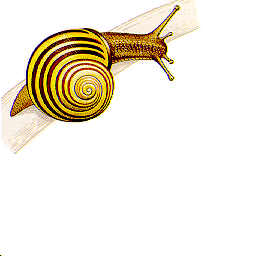
\includegraphics[width=5cm]{figuras/snail.png}
  \fonte{Adaptada de \url{https://people.math.sc.edu/Burkardt/data/bmp/bmp.html}.}
\end{figure}

\section{Métricas de avaliação}

As seguintes métricas foram computadas:

\begin{itemize}
  \item \textbf{Taxa de compressão}: Razão entre o tamanho não comprimido e o tamanho comprimido.
  \item \textbf{Tempo de compressão/descompressão}: medido em segundos.
  \item \textbf{Memória pico}: memória máxima observada durante a execução (MB).
  \item \textbf{Integridade}: verificação de \emph{round trip} (\texttt{decode(encode(x)) == x}).
\end{itemize}

\section{Resultados com a biblioteca \textit{Komm}}

Iniciamos avaliando as implementações já disponíveis na \textit{Komm}: Huffman, Shannon--Fano, Tunstall, LZ78, LZW e LZ77 (com janelas de 4\,kB a 64\,kB). As Figuras~\ref{fig:komm-alice-compression}–\ref{fig:komm-alice-time} apresentam os resultados sobre o texto \textit{Alice}; as Figuras~\ref{fig:komm-smiley-compression}–\ref{fig:komm-smiley-time}, sobre a imagem \textit{smiley}.

\begin{figure}[h]
  \centering
  \caption{Texto \textit{Alice}: taxa de compressão.}
  \label{fig:komm-alice-compression}
  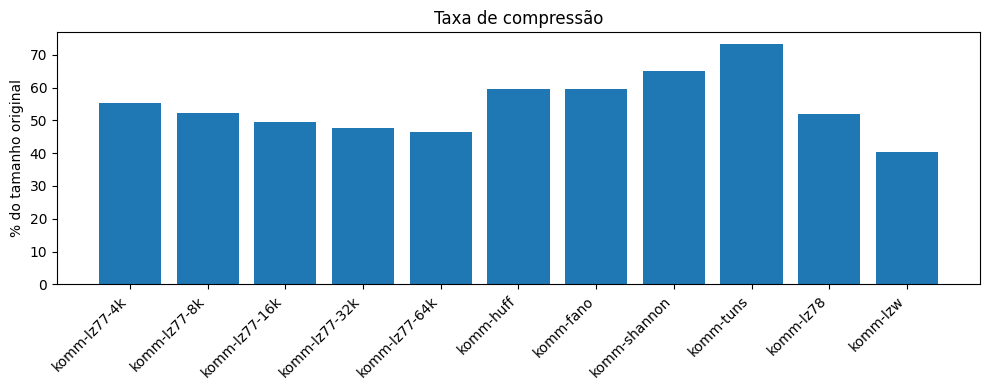
\includegraphics[width=15cm]{figuras/komm_alice_compression.png}
  \fonte{Elaborada pelo autor.}
\end{figure}

\begin{figure}[h]
  \centering
  \caption{Texto \textit{Alice}: memória pico.}
  \label{fig:komm-alice-memory}
  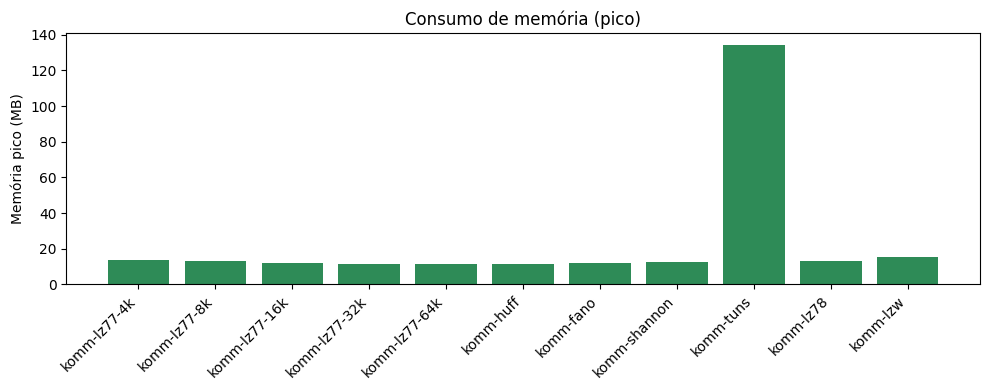
\includegraphics[width=15cm]{figuras/komm_alice_memory.png}
  \fonte{Elaborada pelo autor.}
\end{figure}

\begin{figure}[h]
  \centering
  \caption{Texto \textit{Alice}: tempo de compressão.}
  \label{fig:komm-alice-time}
  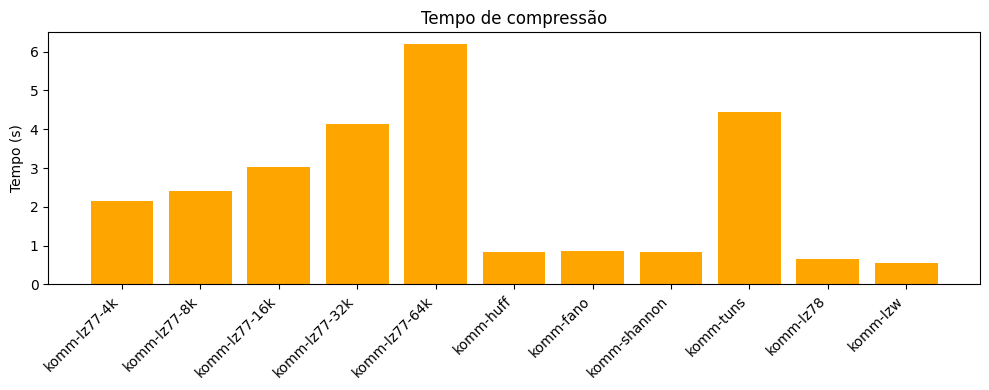
\includegraphics[width=15cm]{figuras/komm_alice_time.png}
  \fonte{Elaborada pelo autor.}
\end{figure}

\paragraph{Principais observações (texto).}
\begin{itemize}
  \item As variantes do \textit{LZ77} exibem o \emph{trade-off} esperado: janelas maiores melhoram a taxa de compressão, com aumento proporcional de tempo e memória.
  \item \textit{Huffman} e \textit{Shannon--Fano} são muito rápidos e leves em memória, com taxas compatíveis com códigos prefixos estáticos.
  \item \textit{Tunstall} demanda mais memória (dicionários extensos), refletindo-se também no tempo.
  \item \textit{LZ78} e \textit{LZW} ficam em um ponto intermediário entre taxa e tempo.
\end{itemize}

\begin{figure}[h]
  \centering
  \caption{Imagem \textit{smiley}: taxa de compressão.}
  \label{fig:komm-smiley-compression}
  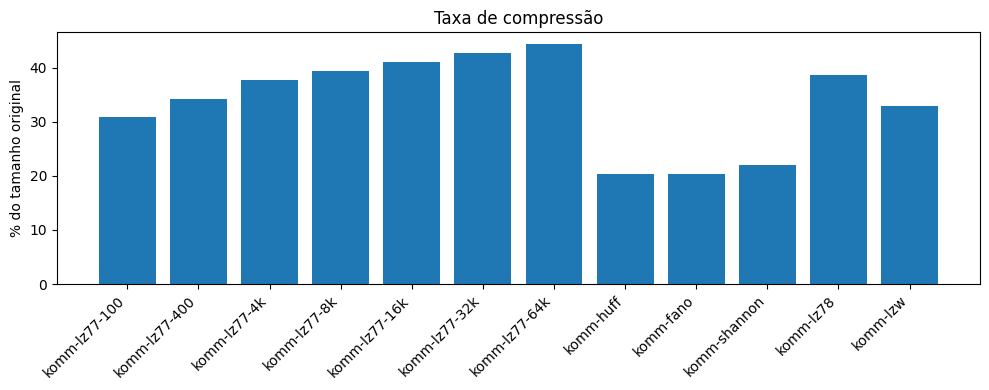
\includegraphics[width=15cm]{figuras/komm_smiley_compression.png}
  \fonte{Elaborada pelo autor.}
\end{figure}

\begin{figure}[ht]
  \centering
  \caption{Imagem \textit{smiley}: memória pico.}
  \label{fig:komm-smiley-memory}
  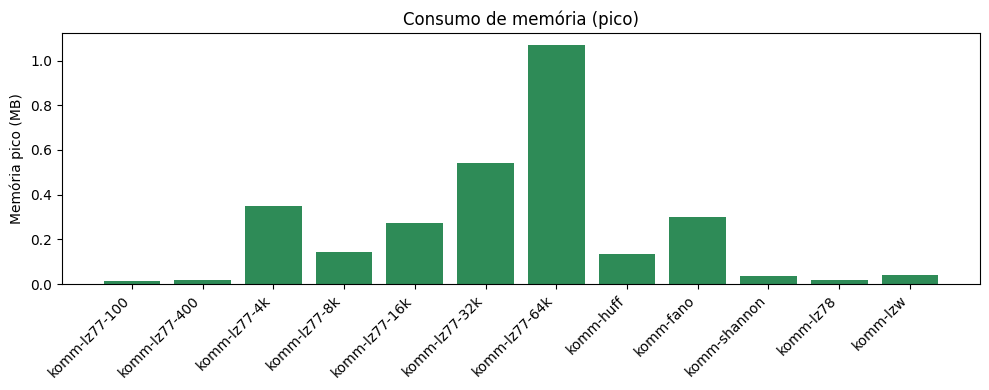
\includegraphics[width=15cm]{figuras/komm_smiley_memory.png}
  \fonte{Elaborada pelo autor.}
\end{figure}

\begin{figure}[ht]
  \centering
  \caption{Imagem \textit{smiley}: tempo de compressão.}
  \label{fig:komm-smiley-time}
  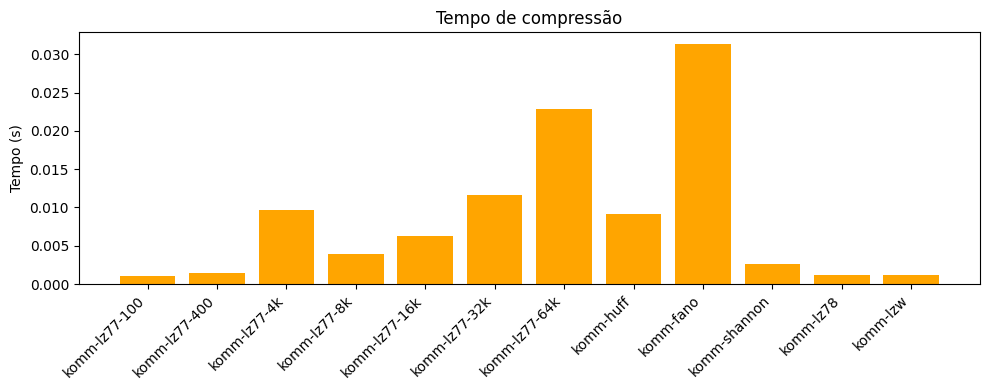
\includegraphics[width=15cm]{figuras/komm_smiley_time.png}
  \fonte{Elaborada pelo autor.}
\end{figure}

\paragraph{Principais observações (imagem).}
\begin{itemize}
  \item Em imagens com grandes áreas uniformes, o LZ77 se beneficia de janelas maiores (maior chance de reutilizar sequências longas).
  \item O custo de tempo/memória cresce com a janela no LZ77, enquanto permanece relativamente estável para Huffman, Shannon--Fano e LZ78/LZW.
\end{itemize}

\begin{quadro}[ht]
\caption{Quadro mostrando uso de memoria e tempo dos algoritmos}\label{quadro:resultados-komm-smiley}
\begin{tabular}{|l|r|r|}
    \hline
    \textbf{Algoritmo de compressão}& \textbf{Tempo (s)}  & \textbf{Pico de Memoria (MB)} \\ \hline
    komm-lz77-4k & 0,0096 & 367,894 \\ \hline
    komm-lz77-8k,97 & 0,0039 & 148,218 \\ \hline
    komm-lz77-16k & 0,0062 & 287,370 \\ \hline
    komm-lz77-32k & 0,0115 & 566,106 \\ \hline
    komm-lz77-64k & 0,0228 & 112,2954 \\ \hline
    komm-huff & 0,0092 & 140,961 \\ \hline
    komm-fano & 0,0313 & 314,210 \\ \hline
    komm-shannon & 0,0026 & 38,195 \\ \hline
    komm-tuns & 3,750 & 15.1985,336 \\ \hline
    komm-lz78 & 0,0011 & 19,928 \\ \hline
    komm-lzw & 0,0011 & 43,084 \\ \hline

\end{tabular}
\fonteproprioautor
\end{quadro}

